\chapter{Nozioni di base}\label{chapter:cap_one_notions}
Prendendo in esame un tessuto qualsiasi, questo viene sezionato e diviso in celle più piccole, dette \textit{spot}.
Uno spot, quindi, non è altro che una posizione pre-definita su una griglia, con un \textit{barcode}\footnote{Una breve sequenza di DNA univoca per ogni spot} che lo identifica.
In genere ogni spot ha un diametro di circa $\qty{55}{\micro\meter}$ e con una distanza da spot a spot di circa $\qty{100}{\micro\meter}$\cite{spotDiameter}.

Possiamo definire l'insieme dei nostri spots nel seguente modo:  
\begin{equation}
	\mathbb{S}=\{s_1,s_2,...,s_n\}
\label{eq:spots}
\end{equation}
dove ogni $\mathbb{S}_i$ è uno spot.

Ogni spot, al suo interno, contiene più cellule. Per questo motivo, ogni spot viene associato ad un vettore di espressione genica che 
da vita alla matrice $X\in \mathbb{R}^{n\times m}$ dove $n$ è il numero di spot e $m$ il numero di geni.
Possiamo definire l'insieme dei nostri geni nel seguente modo: 
\begin{equation}
	\mathbb{G}=\{g_1,g_2,...,g_m\}
\end{equation}
dove ogni $g_i$ è un gene.
Di conseguenza si può definire lo spot $\mathbb{S}_i \in \mathbb{G}^{m}$ come e assegniamo ad ogni 
$\mathbb{S}_i$ il seguente vettore: 
\begin{equation}
	\bigl( x_{i,1}, x_{i,2}, \dots, x_{i,m} \bigr)
\end{equation}
dove $x_{i,j}\in\mathbb{R}$ rappresenta l'espressione del gene $g_j$
allo spot $s_i$, con $1 \le i \le n$.
\begin{figure}[ht]
	\centering
	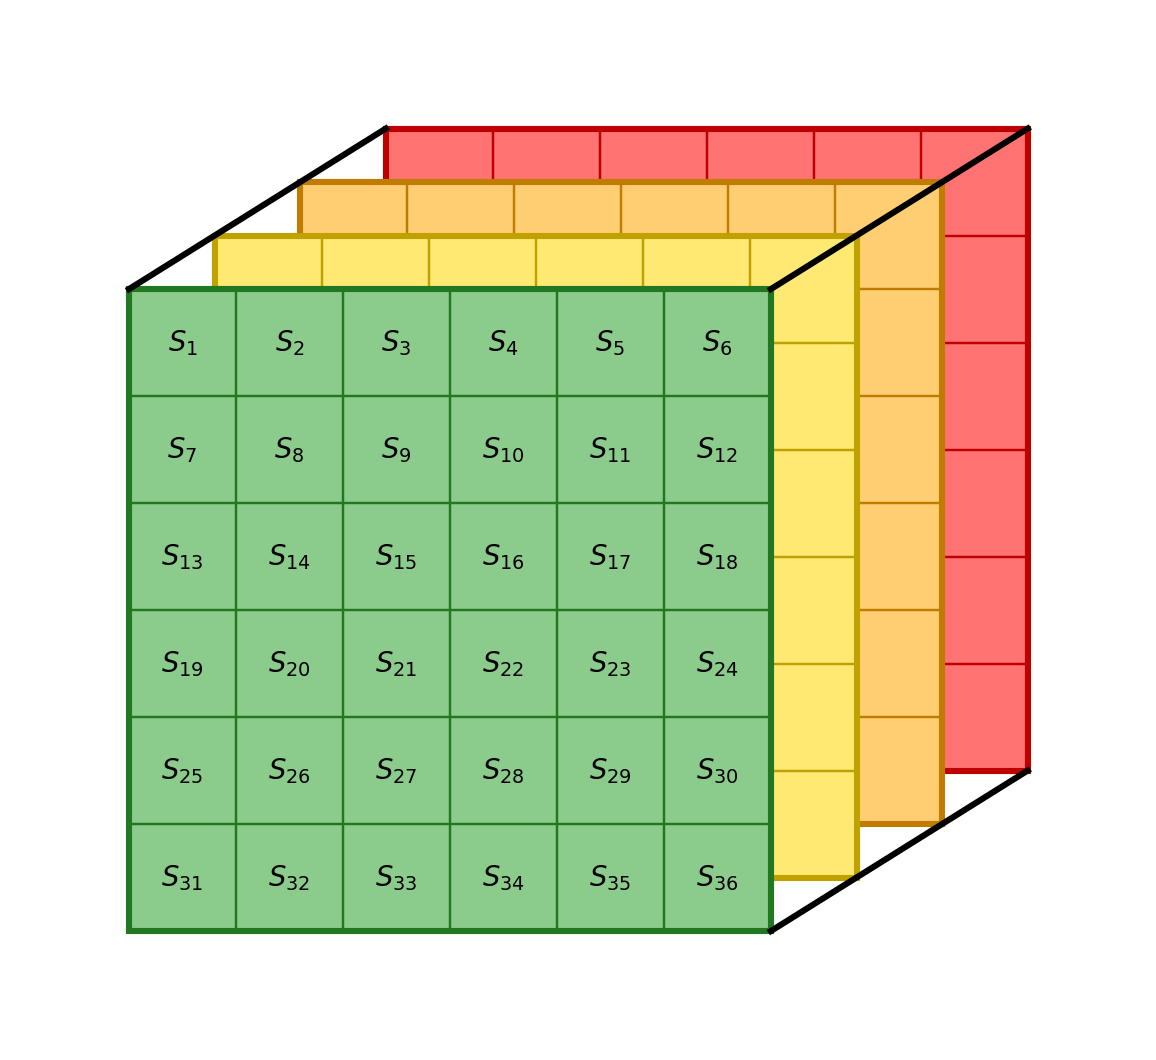
\includegraphics[width=0.575\textwidth]{immagini/spot_cubo.png}
	\caption{Rappresentazione spots e geni}
	\label{fig:four}
\end{figure}

La figura ~\ref{fig:four} mostra una rappresentazione grafica degli spot e dei geni all'interno di un tessuto. Ogni cella rappresenta uno spot, mentre ogni colore rappresenta un gene diverso\footnote{Si noti che il colore non è rappresentativo della presenza o meno di quel gene in quello spot}.
Si può notare che ogni spot $\mathbb{S}_i$, al suo interno, può contenere più geni.
Inoltre, nella figura d'esempio, si hanno 36 spot diversi e 4 geni, ma ma nella realtà i dati
sono differenti: gli spot possono arrivare a oltre 3000
celle e i geni possono superare i 30,000.

La figura \ref{fig:four}, tuttavia, presenta una inesattezza in quanto gli spot non sono disposti su una matrice $n \times n$, bensì hanno una rappresentazione esagonale.
Questo significa che, dato uno spot $\mathbb{S}_i$, questo presenterà sei spot
adiacenti, tranne nei casi in cui gli spot sono localizzati ai bordi del tessuto.

Per poter trovare spazialmente uno spot $\mathbb{S}_i$, quindi, occorre assegnare una coordinata $x$ e una coordinata $y$ ad ogni spot, e, una volta creata una matrice \\$[\mathbb{S}_i, <x_i, y_i>]$,
dove $<x, y>$ indicano le coordinate dello spot, è possibile trovare i 6 vicini attraverso un semplice calcolo.
Inoltre, per sopperire ad eventuali spazi vuoti nel tessuto, viene calcolata la distanza euclidea tra gli spot, in modo da poter scartare gli spot che altrimenti verrebbero erronamente segnati come vicini.

La figura~\ref{fig:five} mostra una rappresentazione grafica degli spot in un tessuto, con le loro coordinate $x$ e $y$.
Lo spot preso in esempio, come riferimento, è lo spot con coordinate $x = 2, y = 3$.
\begin{figure}[ht]
	\centering
	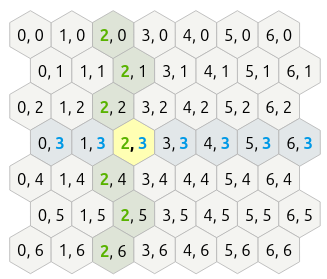
\includegraphics[width=0.5\textwidth]{immagini/spotRappresentazioneEsagonale.png}
	\caption{Rappresentazione spaziale spots}
	\label{fig:five}
\end{figure}

\section{Smoothing spaziale}\label{sec:cap_two_notions}
Quando si entra in possesso di una library, contenente i barcode degli spot, le coordinate spaziali e i relativi metadati, non è consigliato
avviare l'analisi dei dati fin da subito, 
questo perchè i dati di TS contengono anche rumore tecnico e biologico che può mascherare dei pattern in realtà utili, come ad esempio dei geni con profili irregolari.
Occorre quindi prima di tutto ripulire e ridurre la complessità dei dati prima di poterli analizzare.

\medskip
Uno dei primi step per poter poter minimizzare il rumore è applicare un \textit{filtro di media} (Mean Filter),
ovvero una tecnica per poter sostituire ogni elemento, con la media dei valori dei suoi vicini dato un raggio prestabilito\cite{Giotto}.
Questo serve per poter ridurre il rumore locale ed evitare variazioni importanti.

Considerando un tessuto a due dimensioni, contenente $\mathbb{S}$ spots e $\mathbb{G}$ geni.
Possiamo denotare con $y_{ij} \in \mathbb{R}$ il livello di espressione genica di un determinato gene $g_i$ nello spot $\mathbb{S}_i$.
Dalla definizione di matrice di espressione genica $X$ definita precedentemente, possiamo ora definire $\widehat{X}$ la matrice ottenuta come output 
dopo aver applicato la seguente operazione:
\begin{equation}
\hat y_{ij} = \sum_{s_k \in \mathcal{N}_r(s_j)} w_{jk} \cdot y_{ik}
\label{eq:smoothing}
\end{equation}
dove $N_r(s_j) = \{ s_k \mid \| s_k - s_j \| \le r,\; s_k \in \mathbb{S} \}$ con raggio $r \in \mathbb{R}$ denota i vicini dello spot $s_j$, e $w_{jk}$ sono i pesi spaziali 
che soddisfano $\sum_k w_{jk} = 1$.

Per trovare i pesi spaziali poi, viene applicato il filtro di media:
\begin{equation}
	w_{jk} = \frac{1}{\mid \mathcal{N}_r(s_j)\mid}
\label{eq:filtroDiMedia}
\end{equation}
dove $\mathcal{N}_r(s_j)$ denota i vicini dello spot $s_j$ entro il raggio $r$, e tutti i vicini contribuiscono in modo equivalente.

\medskip
\noindent
In alternativa al filtro di media è possibile utilizzare la \textit{Gaussian Kernel Smoothing}\cite{GaussianKernelSmoothing} per calcololare i pesi spaziali.
Prima si devono calcolare i pesi non normalizzati usando un Kernel Gaussiano:
\begin{equation}
	\widetilde w_{jk} = \frac{1}{\sigma\sqrt{2\pi}}\,
\exp\!\left(-\,\frac{\lVert s_k - s_j\rVert^{2}}{2\sigma^{2}}\right)
\label{eq:gaussianKernel}
\end{equation}
dove $\sigma$ controlla la portata spaziale di smoothing.
Dopodichè andremo ad applicare una normalizzazione\footnote{Dividere tutti i termini di un'espressione per uno stesso fattore in modo che l'espressione risultante abbia una certa norma uguale a 1.} per ottenere i pesi finali:
\begin{equation}
	w_{jk} = \frac{\widetilde{w}_{jk}}{\sum_h \widetilde{w}_{jh}}
\label{eq:gaussianKernelNormalization}
\end{equation}
garantendo che $\sum_k w_{jk} = 1$ per ogni spot $s_j$.

\begin{figure}[ht]
	\centering
	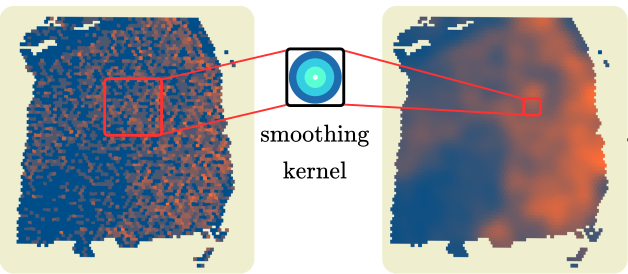
\includegraphics[width=0.8\textwidth]{immagini/spatialSmoothing.png}
	\caption{Dimostrazione di Smoothing Spaziale}
	\label{fig:six}
\end{figure}

La figura \ref{fig:six} dimostra come filtro di media attenua le variazioni locali, riducendo i valori e producendo una mappa più omogenea dove i picchi isolati di rumore risultano smussati.


\medskip
\noindent
\paragraph{Smoothing Spaziale a due fattori}
Un'altra variante allo smoothing visto sopra è lo \textit{smoothing a due fattori}, che combina i vicini spaziali e la loro somiglianza trascrizionale, ovvero i pattern.
Usando lo smoothing a due fattori, i dati smussati risultano essere più accurati nelle loro partizioni e interpretazioni biologiche rispetto all'utilizzo di operazioni a un fattore\cite{smoothingTwoFactors}.

Dato $\mathcal{X}_i$ un vettore di espressione genica per uno spot $i$, 
la sua versione smussata $\mathcal{X}_i'$ può essere calcolata come segue:

\begin{equation}
\mathcal{X}_{i}' = (1-\alpha)\,\mathcal{X}_{i} + \alpha \left(
    \beta \frac{\sum_{j \in {N}_s(i)} c^{s}_{ji}\,\mathcal{X}_{j}}
               {\sum_{k \in {N}_s(i)}\, c_{ki}^s}
    + (1-\beta) \frac{\sum_{j \in {N}_p(i)} c^{p}_{ji}\,\mathcal{X}_{j}}
                      {\sum_{k \in {N}_p(i)}\, c_{ki}^p}
\right).
\label{eq:smoothingTwoFactors}
\end{equation}
Nella equazione \ref{eq:smoothingTwoFactors} ci sono due parametri, $\alpha$ e $\beta$.
La prima  regolarizza il rapporto tra l'espressione originale e quella corretta, 
evitando che l'espressione dello spot in esame risulti eccessivamente smussata.
$\beta$ invece modula il peso relativo dello smussamento basato sulla vicinanza spaziale rispetto a quello basato sui pattern.
$N_s(i)$ e $N_p(i)$ indicano, rispettivamente, i vicini spaziali e i pattern nello spot $i$.
$c^{p}_{ji}$ e $c^{s}_{ji}$ indicano, rispettivamente, il contributo spaziale e quello di pattern dello spot $j$ vicino allo spot in oggetto $i$.
\section{Formato dei dati}\label{sec:cap_three_notions}
I dati del campione di tessuto fornitoci sono in formato \textit{10x Visium}, una piattaforma 
di trascrittomica spaziale che misura l'espressione genica 
su sezioni di tessuto, mantenendo per ogni misura la posizione spaziale. 
La cattura avviene su spot barcodati stampati su una slide. Il programma che processa i dati in modo da mappare i barcode con la loro 
posizione spaziale viene chiamato \textit{Space Ranger} e produce la matrice \textit{Features}$\times$\textit{Barcodes}, dove con Features si intendono i geni, 
e con Barcodes i vari spot; 
Ogni spot raccoglie RNA da più cellule e i conteggi vengono poi mappati sull'immagine.


I file 10x Visium sono in formato \texttt{.h5}, un file specifico pronto per essere elaborato da \texttt{ScanPy} una libreria Python\footnote{Linguaggio di programmazione di alto livello, interpretato e open source}
open-source\footnote{Codice sorgente libero} progettata per l'analisi di dati di trascrittomica.
Scanpy infatti offre la funzione \texttt{sc.read\_visium()} per importare direttamente le cartelle di output di Space Ranger.

Prendendo il file \texttt{.h5} e traducendolo in un file \texttt{.tsv} (Tab-Separated Values) si può osservare una struttura di questo tipo:
\begin{table}[H]
\centering
\caption{Estratto metadati spot (dataset \texttt{1.DLPFC}).}
\label{tab:tsvTable}
\resizebox{\textwidth}{!}{%
\begin{tabular}{lcccc}
\hline
\textbf{Barcode} & \textbf{Row} & \textbf{Col} & \textbf{Cluster} & \textbf{sum\_Gene} \\
\hline
AAACAAGTATCTCCCA-1 & 1 & 3 & 7 & 3586 \\
AAACAATCTACTAGCA-1 & 1 & 27  & 4 & 1150 \\
AAACACCAATAACTGC-1 & 1 & 59 & 8 & 1960 \\
\hline
\end{tabular}%
}
\end{table}
\begin{minipage}{\textwidth}
\centering
\label{tab:legendTsvTable}
\footnotesize
\texttt{barcode}: identificatore dello spot;\;
\texttt{sample\_name}: nome del campione;\;\\
\texttt{row}, \texttt{col}: coordinate dello spot nella griglia;\;\\
\texttt{Cluster}: cluster di appartenenza;\;
\texttt{sum\_gene}: numero totale di geni rilevati.
\end{minipage}

La tabella \ref{tab:tsvTable} è solo una sezione di cosa contiene davvero il file \texttt{.h5}, nella realtà sono presenti svariagi gigabyte di dati.

Oltre ai file sopracitati viene fornita anche una cartella chiama \texttt{spatial} contenente immagini ad alta e bassa definizione 
del tessuto, e il file delle posizioni degli spot chiamato \texttt{tissue\_positions.csv}

\begin{figure}[ht]
	\centering
	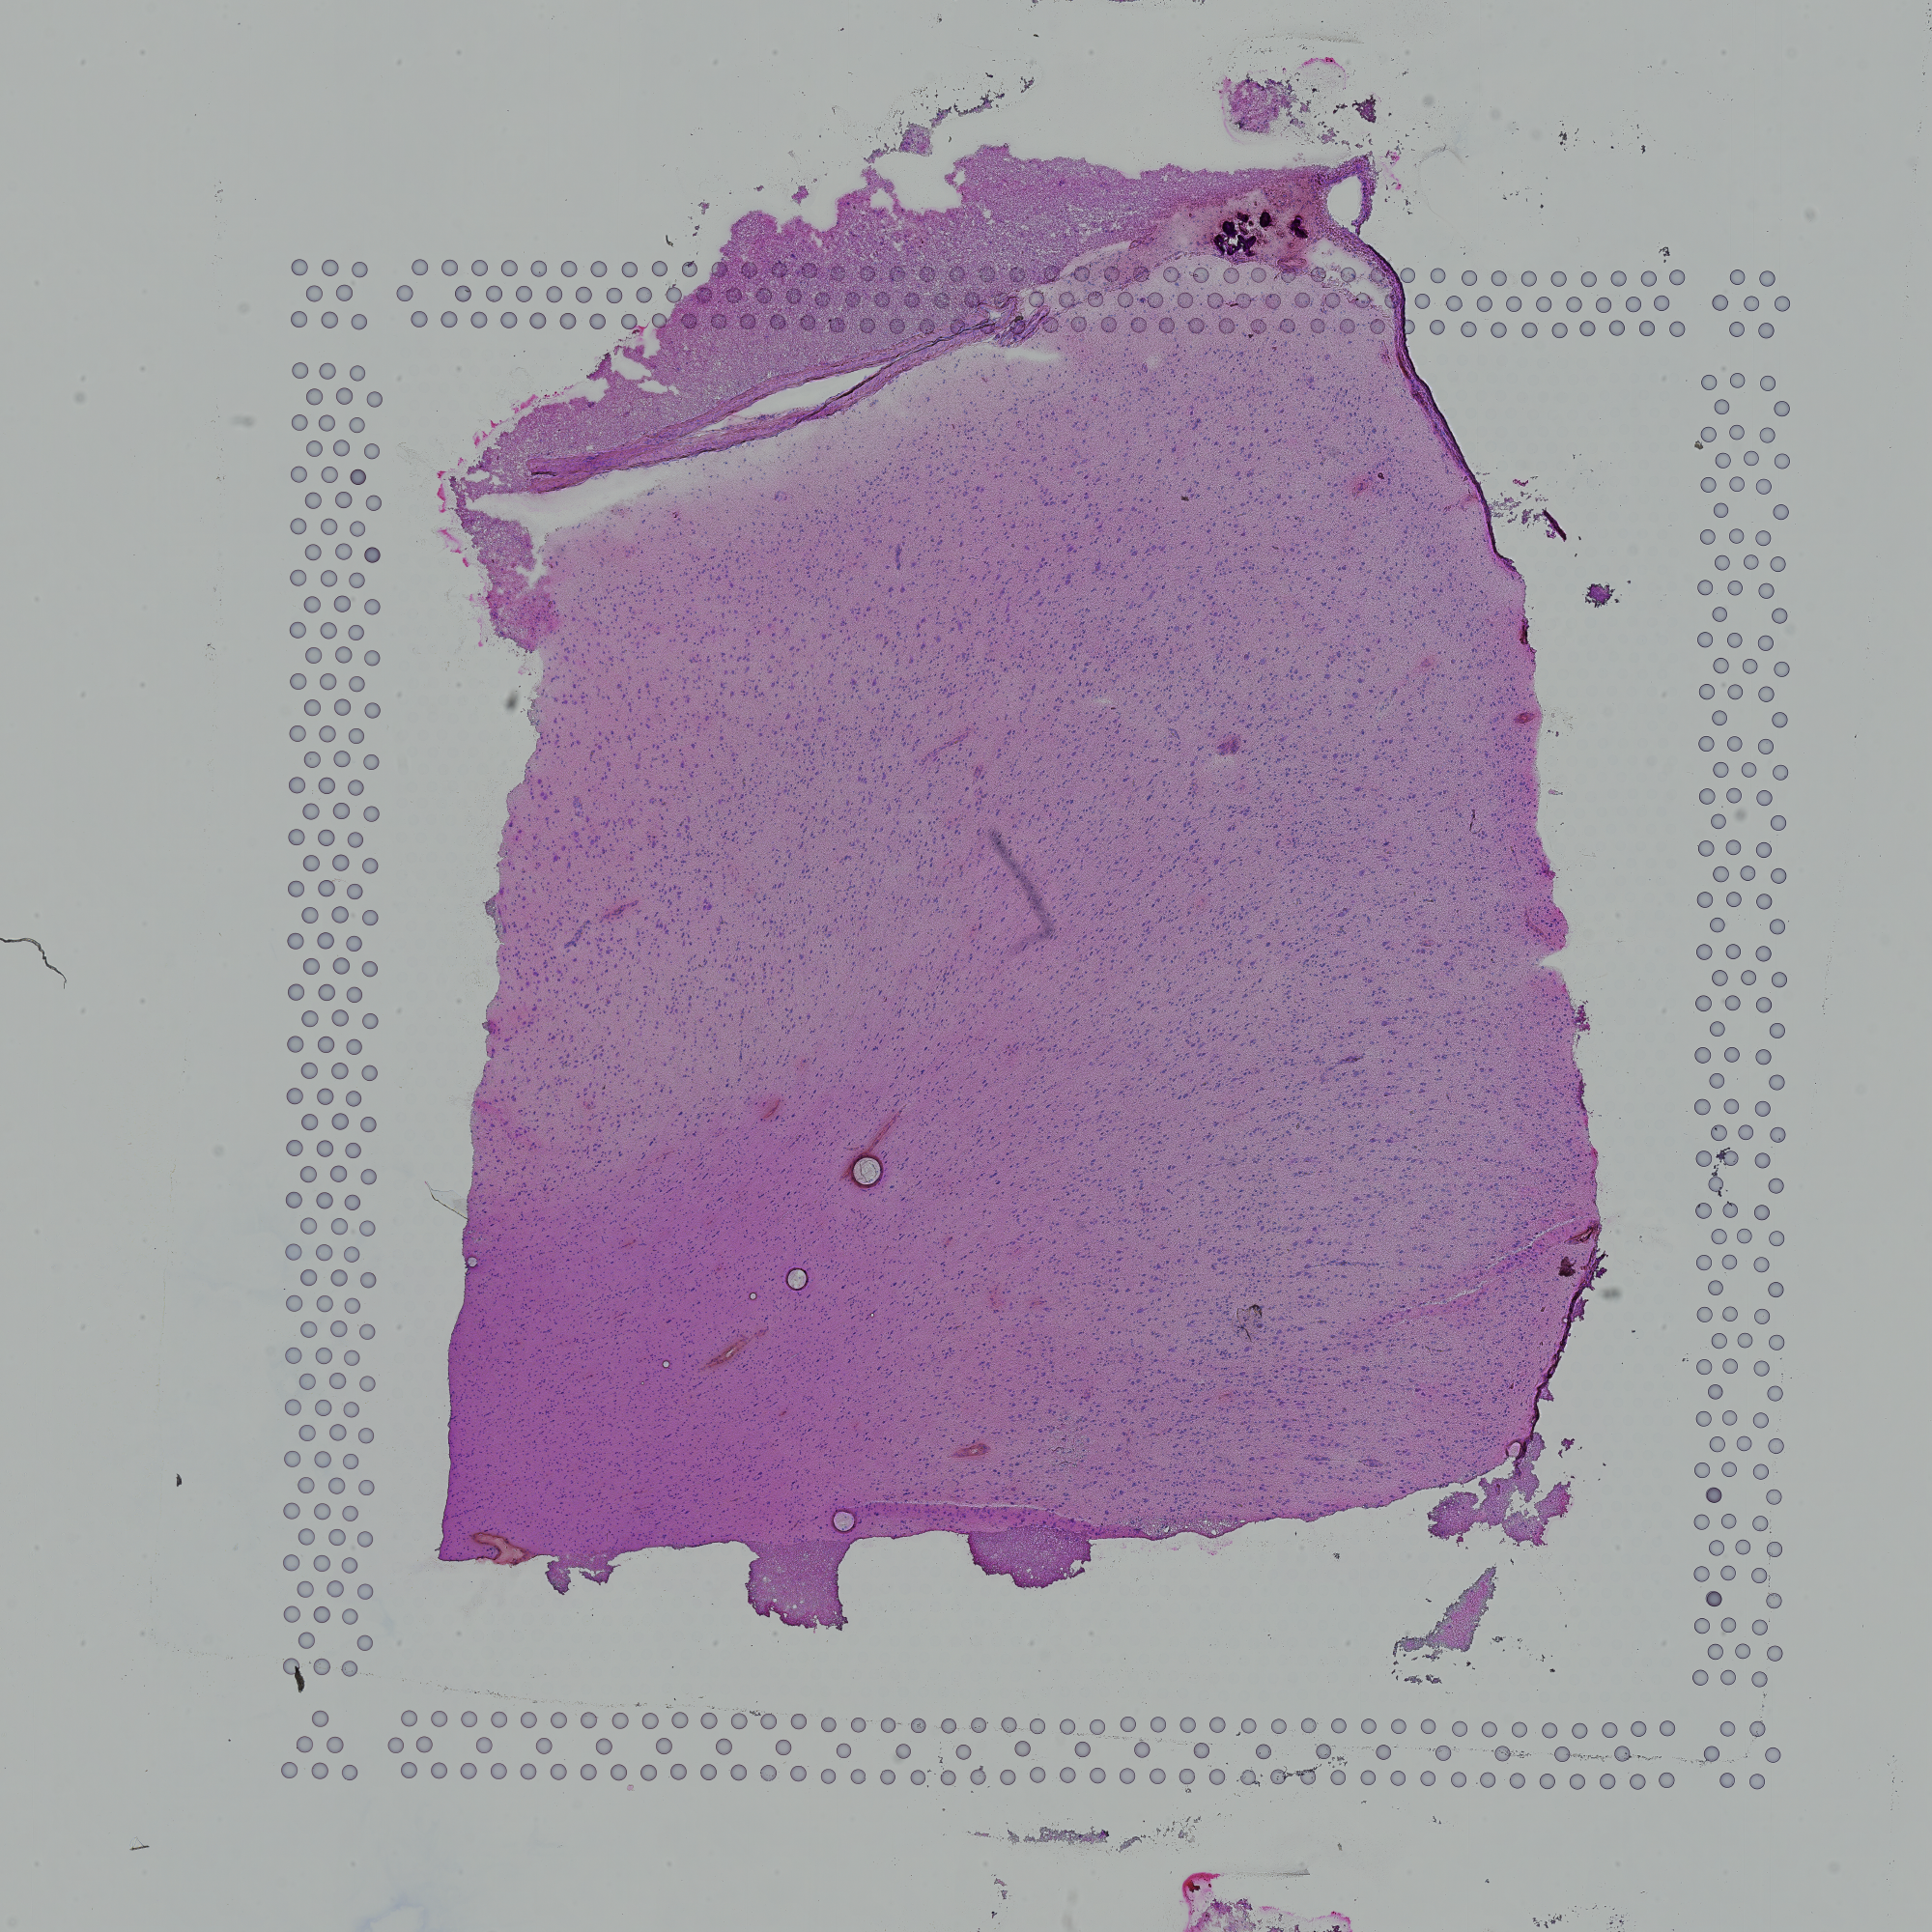
\includegraphics[width=0.8\textwidth]{immagini/tissue_hires_image.png}
	\caption{File che contiene la foto del tessuto: \texttt{tissue\_hires\_image.png}}
	\label{fig:seven}
\end{figure}

\section{Scanpy}\label{sec:cap_four_notions}
Scanpy è un toolkit in Python per l'analisi di dati di espressione genica a singola cellula, 
progettato per lavorare anche con dataset molto estesi e per integrarsi con l'ecosistema Python. 
Include metodi per il pre-processing, come filtri su cellule e geni, normalizzazione, identificazione degli HVGs e clustering. 

Scanpy fornisce inoltre funzioni con velocità elevate che rendono l'analisi di 
data set con più di un milione di cellule e interrogazioni real time nell'ordine di secondi per data set con circa 100,000 cellule.
Questa moltitudine di funzioni, assieme ad velocità non indifferente, ne hanno favorito l'adozione in molti ambiti di ricerca.\cite{scanPyUsage}

Dal punto di vista della manutenibilità invece, Scanpy è sviluppato nell'mbito del progetto \textit{scverse}, 
che coordina strumenti fondamentali per l'analisi omica in Python. 
Questo garantisce linee guida comuni, interoperabilità tra pacchetti e una documentazione unificata, 
elementi cruciali in contesti accademici e clinici dove la tracciabilità delle analisi è essenziale.\cite{scverse}

\medskip
\noindent
Le funzioni della libreria sono organizzate per famiglie:
\begin{itemize}
	\item \texttt{sc.pp.*} rigurda le varie funzioni per il pre-processing.
	\item \texttt{sc.tl.*} serve per gli strumenti analitici, come clustering o creazione di grafi.
	\item \texttt{sc.pl.*} infine riguarda le varie funzioni usate per la visualizzazione, con cui è possibile stampare a video delle immagini.
\end{itemize}

\noindent
Per la trascrittomica spaziale, 
Scanpy offre un'integrazione naturale con i dati 10x Visium tramite 
\texttt{scanpy.read\_visium()}, che carica non solo la matrice di espressione ma anche immagini e coordinate degli spot. 
La funzione ha la seguente firma:

\begin{center}
\begin{minipage}{8cm}
\begin{verbatim}
scanpy.read_visium(
    path,
    genome = None,
    count_file = 'filtered_feature_bc_matrix.h5',
    library_id = None,
    load_images = True,
    source_image_path = None
	)
\end{verbatim}
\end{minipage}
\end{center}

\noindent
Gli argomenti della funzione sono i seguenti:
\begin{itemize}
  \item \texttt{path}: Percorso alla cartella radice che contiene l'output Visium, ovvero il file \texttt{.h5} e la sottocartella \texttt{spatial/}.
  \item \texttt{genome}: Opzionale, è lidentificatore del genoma che si vuole filtrare, se presente nei metadati 10x.
  \item \texttt{count\_file}: Nome del file di 10x Visium contenente i vari dati. Deve essere presente nella cartella inserita in \texttt{path}. Di default ha come nome (\texttt{filtered\_feature\_bc\_matrix.h5} per default.
  \item \texttt{library\_id}: Opzionale, e l'dentificativo della libreria Visium. Risulta utile quando occorre concatenare più librerie.
  \item \texttt{load\_images}: Se \texttt{True}, carica le immagini del tessuto.
  \item \texttt{source\_image\_path}: Opzionale, è il percorso alternativo da cui leggere le immagini se non si trovano in \texttt{spatial/}.
\end{itemize}

\noindent
La funzione restituisce un oggetto \texttt{AnnData}, una struttura dati che accoppia in modo coerente la matrice di espressione con annotazioni su spot 
e geni, oltre che a campi dedicati per grafi e metadati.
\texttt{anndata.X} contiene la matrice \textit{Features}$\times$\textit{Barcodes}, \texttt{anndata.obs} da \textit{Observations} contiene tutti e solo i barcodes degli spot, mentre 
\texttt{anndata.vars} da \textit{Variables} contiene tutti e solo i geni misurati, con nome, id e tipo.
Gli oggetti \texttt{AnnData} si possono salvare tramite la funzione \texttt{anndata.write\_h5ad()} e i file così creati hanno estensione \texttt{.h5ad}.

\medskip
\noindent
La funzione sopracitata ha la seguente firma:
\begin{center}
\begin{minipage}{8cm}
\begin{verbatim}
anndata.write_h5ad(
		filename,
		compression = hdf5plugin.FILTERS["zstd"]
	)
\end{verbatim}
\end{minipage}
\end{center}

\noindent
Con come argomenti: 
\begin{itemize}
  \item \texttt{filename}: Il nome del file che si vuole salvare con estensione \texttt{.h5ad}.
  \item \texttt{compression}: Opzionale, metodi alternativi di compressione del file.
 \end{itemize}

Un esempio completo di un programma scritto in linguaggio Python con lettura dei dati 10x Visium attraverso Scanpy e 
relativo salvataggio di AnnData in formato \texttt{.h5ad} è il seguente:

\begin{lstlisting}[style=mypython, caption={Funzione per caricare il file \texttt{.h5} ed esempio su come utilizzarla per inizializzare oggetto \texttt{AnnData}}]
import scanpy as sc

def load_data():
    
    adata_gene_expression = sc.read_visium("1.DLPFC/151673", count_file="filtered_feature_bc_matrix.h5", load_images=True)
    
    return adata_gene_expression

annData = load_data()

annData.write_h5ad(filename="processed_adata")
\end{lstlisting}

\section{Ottenimento Maschere Binarie dei geni}\label{cap:BinaryMasks}
Una volta ottenuti i dati in formato \texttt{AnnData} è possibile iniziare a manipolarli come oggetto per poterne ricavare le varie informazioni 
necessarie allo studio che si sta svolgendo.

Come detto in precendeza occorre applicare prima di tutto uno Smoothing per poter ripulire e ridurre la complessità dei dati ottenuti.
Questo smoothing viene applicato gene per gene attraverso il filtro di media, definito precedentemente, in questo modo:
\begin{lstlisting}[style=mypython,label=code:MeanFilter,caption={Funzioni per ottenere i dati di un gene specifico e applicarci il filtro di media}]
	ITNI = np.zeros((nspot, 7), dtype=int)
	VNI   = (ITNI!=-1).astype(int)
    NN    = VNI.sum(axis=1)
    NM    = (VNI.T / NN.T).T

	def get_gene_data(data, gene_id):
		array_data = data.X.toarray().T
		gene_data  = array_data[gene_id]
		return gene_data
	
	def super_opt_mean_filter(gene_data):
		global ITNI, NM
		return (gene_data[ITNI] * NM).sum(axis=1)

	def opt_mean_filter_iterated(gene_data, it):
		for _ in range(it):
			gene_data = super_opt_mean_filter(gene_data)
		return gene_data
	
	geneData = get_gene_data(anndata, 1)

	geneData = opt_mean_filter_iterated(gdata, 5)
\end{lstlisting}

Lo Snippet del codice \ref{code:MeanFilter} presenta 3 funzioni principali che permettono di utilizzare il filtro di media: la prima, 
\texttt{get\_gene\_data(data, gene\_id)}, permette di recuperare dall'oggetto \texttt{AnnData} un gene dato il suo \texttt{id}.
Il suo funzionamento è molto basico in quanto intuitivamente viene creata una variabile contenente la matrice trasposta di \texttt{AnnData.X}, che, come detto precedentemente, l'oggetto \texttt{X} 
all'interno di \texttt{AnnData} contiene la matrice \textit{Features}$\times$\textit{Barcodes}, e rendendola trasposta essa viene trasformata in \textit{Barcodes}$\times$\textit{Features}, ovvero anzichè avere 
in ogni riga uno spot e per ogni colonna l'espressione genica di un determinato gene su quello spot, si otterrà invece un gene per ogni riga, e la sua espressione genica su ogni spot per ogni colonna.
La tabella \ref{tab:ann_data_and_transpose} contiene una rappresentazione visiva della matrcie \texttt{AnnData.X} e della sua relativa trasposta.

\begin{table}[htbp]
  \centering
  \caption{Struttura di \texttt{AnnData.X} e della sua trasposta}
  \label{tab:ann_data_and_transpose}
  
  \textbf{Matrice $X = \texttt{AnnData.X}$} \\[0.5em]
  \begin{tabular}{c|ccc}
    & Gene1 & Gene2 & Gene3 \\
    \hline
    Spot1 & $0$ & $10$ & $24$ \\
    Spot2 & $15$ & $2$ & $0$ \\
    Spot3 & $14$ & $12$ & $23$ \\
  \end{tabular}

  \vspace{2em} 

  \textbf{Trasposta $X^\top$} \\[0.5em]
  \begin{tabular}{c|ccc}
    & Spot1 & Spot2 & Spot3 \\
    \hline
    Gene1 & $0$ & $15$ & $14$ \\
    Gene2 & $10$ & $2$ & $12$ \\
    Gene3 & $24$ & $0$ & $23$ \\
  \end{tabular}
  
\end{table}


La seconda funzione, \texttt{super\_opt\_mean\_filter(gene\_data)}, implementa un filtro di media sui valori di espressione genica sfruttando operazioni completamente vettorizzate.
Prima della funzione vengono definite alcune variabili di supporto:

\begin{itemize}
\item \texttt{ITNI}: matrice di forma $(n_{spot}, 7)$ contenente, per ogni spot, gli indici dei suoi vicini. Gli elementi pari a \texttt{-1} indicano assenza di vicino.
\item \texttt{VNI = (ITNI != -1)}: maschera binaria che vale $1$ dove l'indice è valido e $0$ altrimenti.
\item \texttt{NN = VNI.sum(axis=1)}: numero di vicini validi per ciascuno spot.
\item \texttt{NM = (VNI.T / NN.T).T}: matrice di pesi normalizzati, dove ogni vicino valido riceve un peso pari a $\frac{1}{NN_i}$.
\end{itemize}

La funzione calcola la media dei valori di espressione di un gene sui vicini di ciascuno spot.
Ogni riga della matrice \texttt{gene\_data[ITNI]} contiene i valori del gene nei vicini di uno spot, che vengono moltiplicati per i pesi corrispondenti in \texttt{NM} e poi sommati.
Il risultato è un vettore in cui ogni elemento rappresenta la media dei valori di espressione nei vicini.

La terza funzione, \texttt{opt\_mean\_filter\_iterated(gene\_data, it)}, semplicemente itera \texttt{it} volte la funzione precedente.
Questo perchè iterando più volte il filtro di media, ottengo una rappresentazione più accurata del valore dei vicini di ogni gene, e quindi ottenendo una rappresentazione migliore delle zone più dense.
\newline

\begin{figure}[ht]
	\centering
	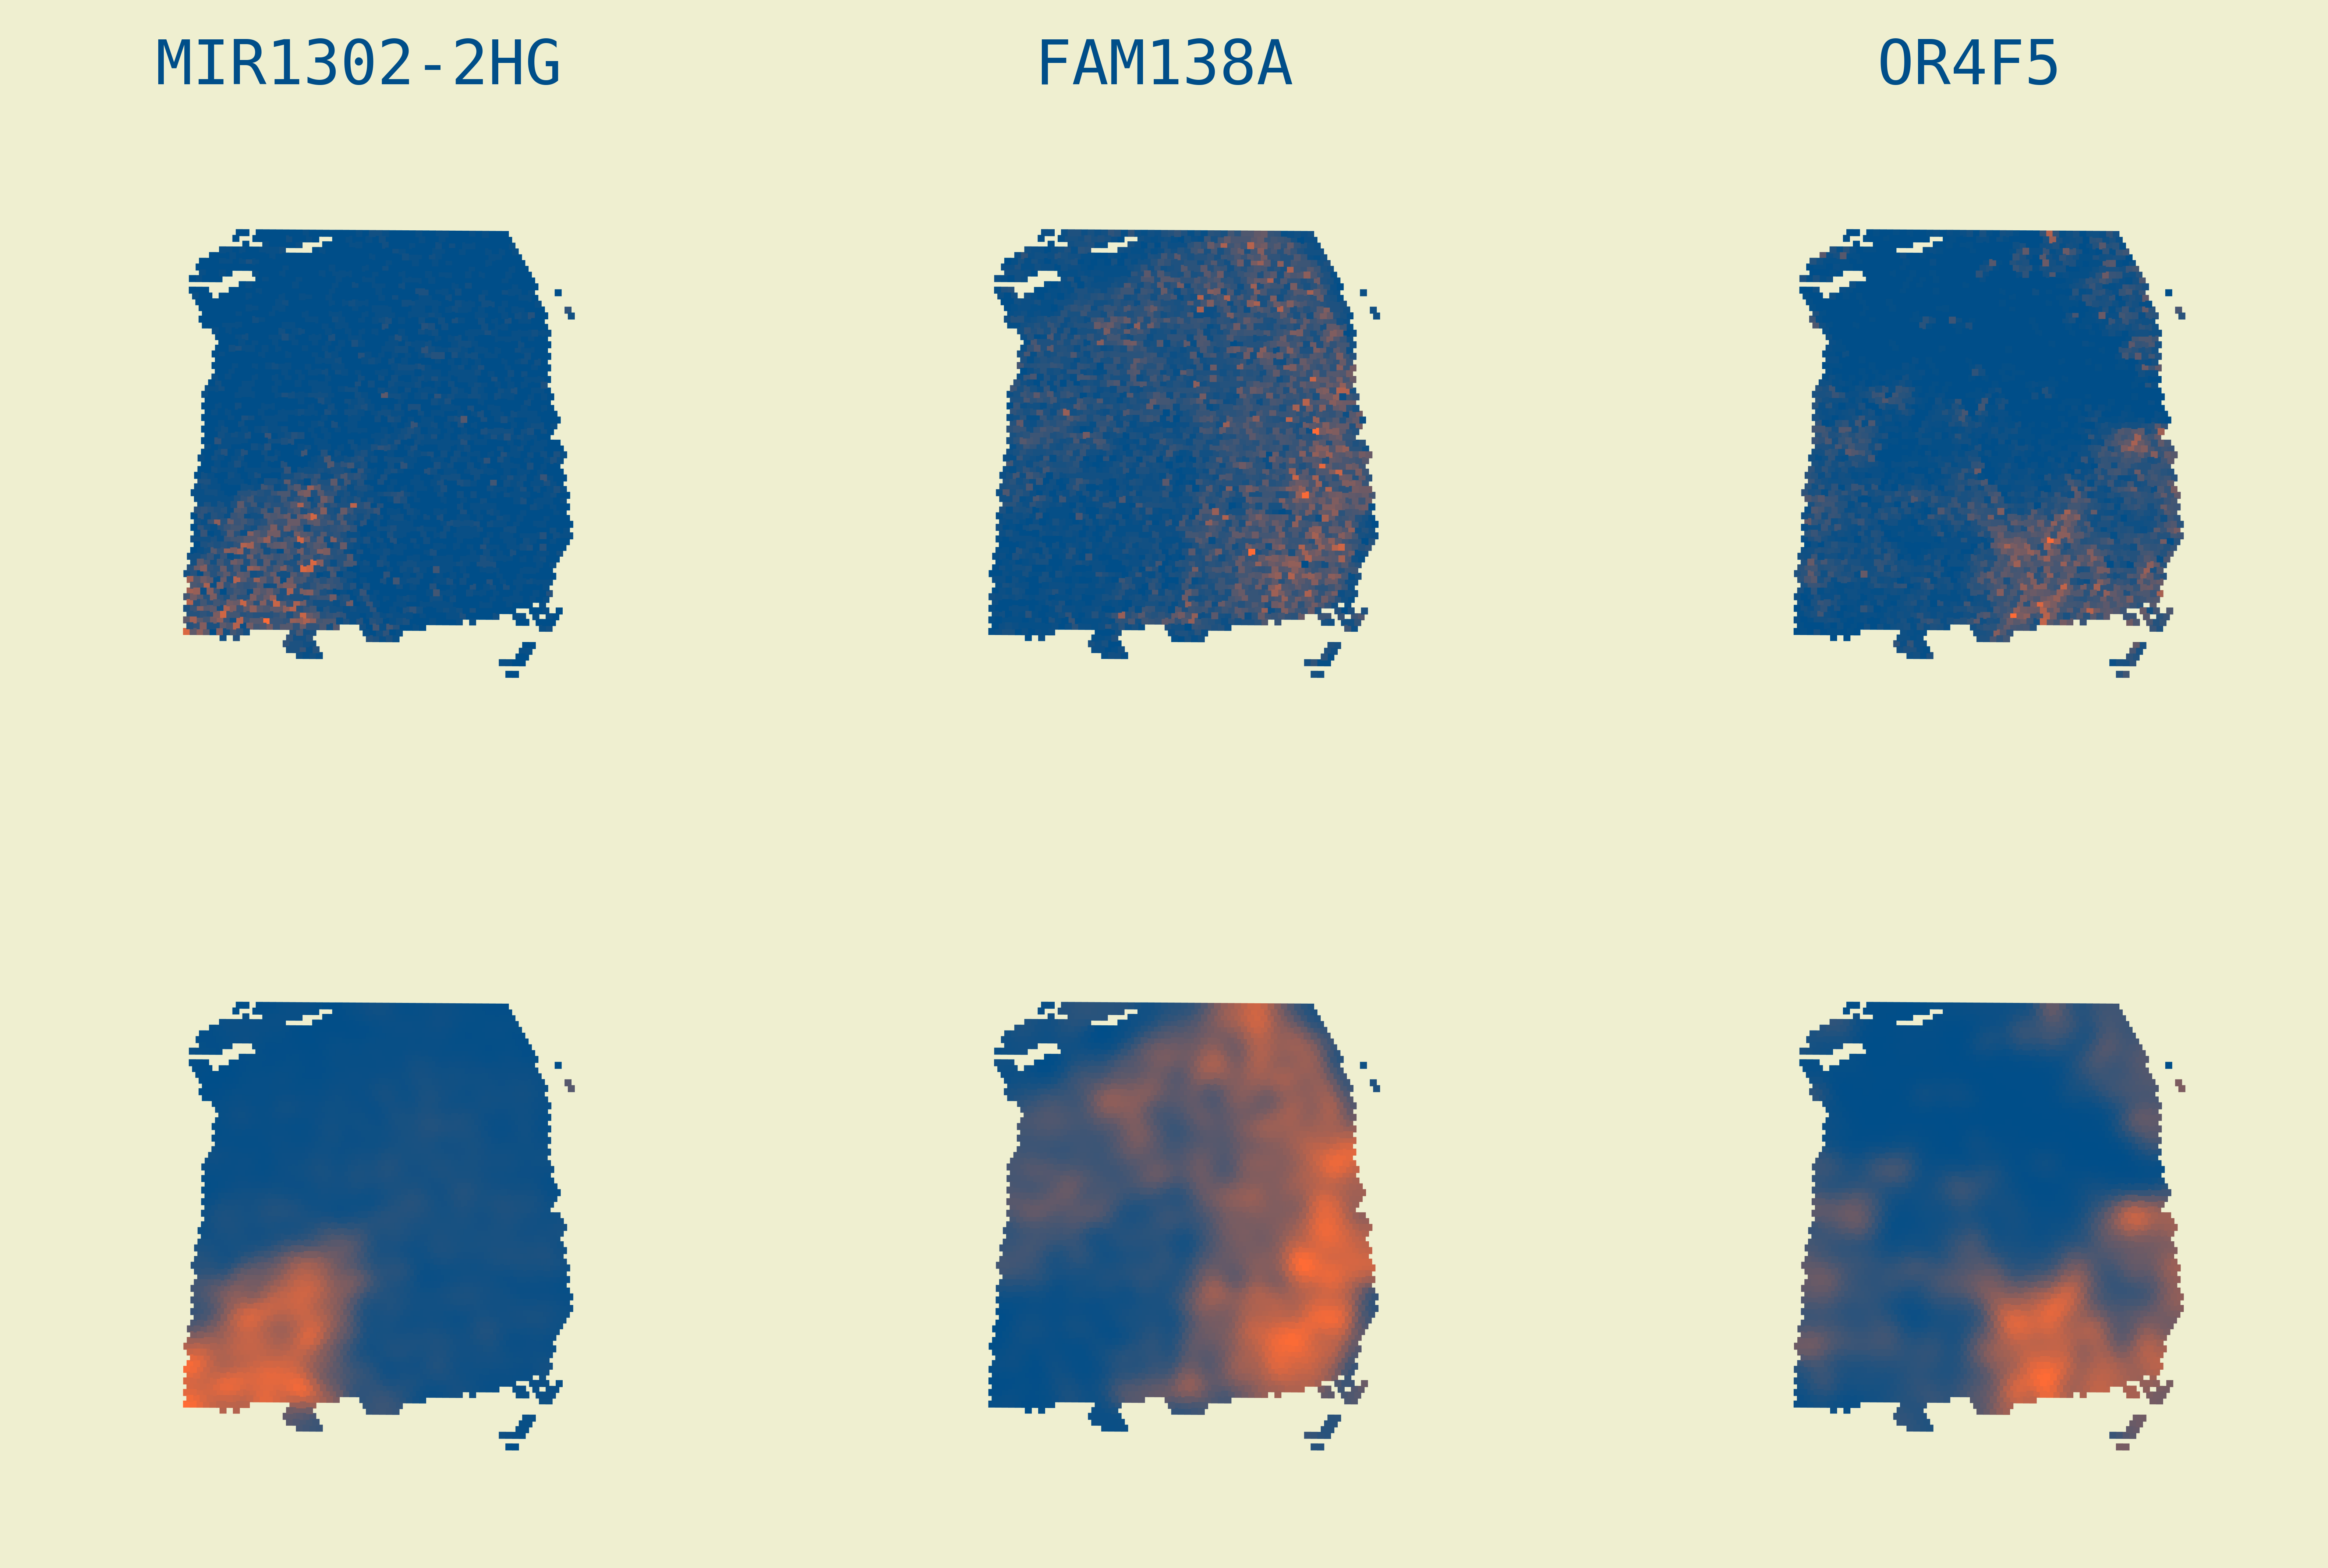
\includegraphics[width=0.8\textwidth]{immagini/mean_filter.png}
	\caption{Rappresentazione di alcuni geni prima e dopo il filtro di media}
	\label{fig:meanFilter}
\end{figure}

Una volta ottenuto i vari geni con le loro espressioni geniche "smussate" dal filtro di media, stimiamo per ogni gene 
un modello di misura  $\forall k \text{ tale che } 1 \le k \le 10$ gaussiane, attraverso la funzione di \texttt{sklearn.mixture.GaussianMixture()}.
Questo algoritmo cerca di adattare, per ciascun valore di $k$, 
una combinazione\footnote{In inglese: mixture} di $k$ distribuzioni gaussiane 
ai dati di espressione del gene in esame, al fine di modellare la presenza di sottopopolazioni 
o modalità multiple nell'espressione. 

\begin{figure}[ht]
	\centering
	
\includegraphics[width=1\textwidth]{immagini/gauss_misxture_multik.png}
	\caption{Dimostrazione di come diverse $k$ rappresentano diversamente i dati}
	\label{fig:gaussianMixture}
\end{figure}

Si può osservare dalla figura \ref{fig:gaussianMixture} come con $1 \le k$ la rappresentazione non colga efficacemente ogni picco dell'espressione genica del gene preso in esame; Si verifica perciò un fenomeno di \textit{underfitting}\footnote{Modello troppo semplice per catturare la complessità dei dati}.
Al contario, con $k \> 3$ si verifica il problema opposto, ovvero ho troppe gaussiane per rappresentare efficacemente i dati in oggetto, si verifica perciò dell'\textit{overfitting}.
Nell'esempio della figura \ref{fig:gaussianMixture} perciò la $k$ corretta corrisponde a $k = 3$.

Per poter scegliere in autonomia la $k$ corretta, 
una volta allenata la funzione \texttt{sklearn.mixture.GaussianMixture()} con un gene, 
si salva attraverso la funzione \texttt{GaussianMixture().bic()} il \textit{Bayesian Information Criterion}(BIC) corrispondente a tale $k$ su quel gene.
Il BIC è un indice statistico che misura quanto bene un modello spiega i dati passati, 
penalizzando i modelli troppo complessi.

La formula con la quale si può ottenere è la seguente:
\begin{equation}
	\mathrm{BIC} = k \cdot \ln(n) - 2 \cdot \ln(\widehat{L})
\end{equation}
dove $n$ indica il numero degli spots, $k$ il numero di parametri stimati dal modello, $\widehat{L}$ massima verosimiglianza del modello, 
ovvero quanto bene il modello si adatta ai dati.

Una volta ottenuti i vari BIC per ogni $k$, viene infine scelta la $k$ corretta attraverso il calcolo del "Knee Point".
Il Knee Point, altro non è che il punto in cui la curva cambia inclinazione in modo evidente, 
passando da una salita marcata a una più piatta, o viceversa.

\begin{figure}[ht]
	\centering
	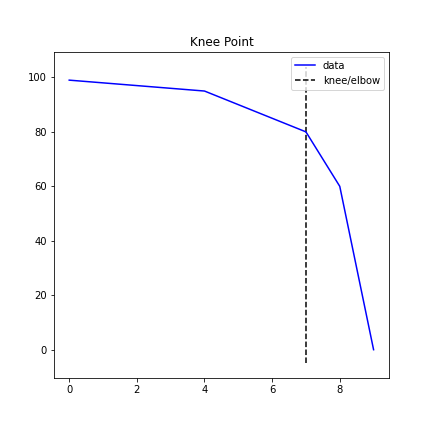
\includegraphics[width=0.6\textwidth]{immagini/kneeOfACurve.png}
	\caption{Esempio di Knee Point}
	\label{fig:kneePoint}
\end{figure}

\noindent
Il codice Python per poter calcolare relativi BIC e Knee Point è il seguente:

\begin{lstlisting}[style=mypython,label=code:gmmAndKnee,caption={Funzioni per ottenere BIC e KP}]
	def gmm_BIC(gdata, mink=2, maxk=10):

		data = gdata.reshape(-1, 1)
		bics = []

		for i in range(mink, maxk+1):
			gmm = GaussianMixture(n_components=i, 
								  random_state=0)
								  	.fit(data)
			BIC_gmm = gmm.bic(data)
			bics.append(BIC_gmm)

		return bics
	
	def find_knee(x, y):
		knee_locator = kneed
						.KneeLocator(
							x, 
							y, 
					 		interp_method="polynomial", 
							curve="convex", 
							direction="decreasing")
		knee   = knee_locator.knee  
			
		return knee
	
	mink = 1
	maxk = 10
	x    = np.arange(mink, maxk+1)
	
	bics = gmm_BIC(gdata, mink, maxk)
	k    = find_knee(x, bics, plt.gca())
\end{lstlisting}

Una volta ottenuta la $k$ ottimale tramite il Knee Point, si può creare la
maschera binaria per il gene in esame. 
La maschera binaria identifica, per ogni spot, se il gene è espresso (1) oppure no (0), 
in base alla soglia determinata dal modello Gaussian Mixture.
Il procedimento è il seguente:
\begin{enumerate}
	\item Si allena il modello GaussianMixture con $k$ componenti sul vettore di espressione genica smussato.
	\item Si assegna ogni spot alla componente gaussiana con la media più alta, presenza del gene, oppure più bassa, assenza.
	\item Si crea la maschera binaria: 1 se lo spot appartiene alla componente con media maggiore, 0 altrimenti.
\end{enumerate}

Questo procedimento mi porterà ad avere un array, di lunghezza \texttt{len($n_{\text{spots}}$)} in cui avrò valore 1 se il gene risulta presente nello spot $s_i$, oppure 0,  con $1 \le i \le s_n$.
\newpage
Il codice per generare la maschera binaria è il seguente:
\begin{lstlisting}[style=mypython,label=code:binaryMask,caption={Funzioni per ottenere le machere binarie una volta ottenuta la k del Knee Point}]
	def fit_MoG(gdata, k):
		data = gdata.reshape(-1, 1)
		gmm  = GaussianMixture(n_components=k,
							   random_state=0)
							   		.fit(data)
		mus  = gmm.means_
		stds = np.sqrt(gmm.covariances_)
		return mus, stds

	def smallest_dist(mus, stds):
    	idx = np.argmin(mus)
    	return mus[idx][0], stds[idx][0][0]
	
	def expansion_filter(gene_data):
		global ITSNI, HNN
		active_neigh = gene_data[ITSNI].sum(axis=1)
		return (active_neigh >= 3)
					.astype(int) * 
					 gene_data + 
					 (active_neigh > 3)
						.astype(int) * 
						 (1-gene_data)

	def expansion_filter_iterated(gene_data, it):
		for _ in range(it):
			gene_data = expansion_filter(gene_data)
		return gene_data
	
	ITSNI = ITNI[:,1:]
    HNN   = NN//2
	mus, stds = fit_MoG(gdata, k)
    m, v = smallest_dist(mus, stds)
    pgdata = expansion_filter_iterated((gdata>(m+1.5*v))
									  	.astype(int), 10)
\end{lstlisting}


Segue la spiegazione di quanto avviene nel codice \ref{code:binaryMask}:

\begin{itemize}
	\item La funzione \texttt{fit\_MoG()} riceve il vettore di espressione smussata \texttt{gdata} e il numero di componenti $k$ trovate dal Knee Point. Viene poi trasformata in colonna da \texttt{gdata.reshape(-1,1)} per adattarsi al modello GaussianMixture. Il modello viene addestrato e restituisce i vettori di medie \texttt{mus} e deviazioni standard \texttt{stds} delle gaussiane. 
  	\item \texttt{smallest\_dist} seleziona la gaussiana con la media più bassa, salvandola nell'indice \texttt{idx}, assumendo che quella rappresenti l'assenza di espressione. Restituisce poi la media $m$ e la deviazione standard $v$ di quella componente.
	\item Nella codice \texttt{gdata > (m + 1.5 * v)).\text{astype(int)}} passato come argomento alla funzione \texttt{expansion\_filter\_iterated}
		si applica la soglia $m + 1.5\cdot v$ per trasformare i valori continui in una prima maschera binaria grezza: gli spot con espressione maggiore rispetto a quella soglia sono considerati attivi, $1$, altrimenti inattivi, $0$.
	\item \texttt{expansion\_filter} raffina questa maschera binaria guardando i vicini: 
		\begin{itemize}
			\item Si calcola il numero di vicini attivi per ciascun spot (\texttt{active\_neigh}).  
			\item Se un vicino ha almeno 3 vicini attivi, si mantiene il valore attuale (\(\texttt{* gene\_data}\)).  
			\item Se ha più di 3 vicini attivi, si può invertire il valore dello spot (\(1 - \texttt{gene\_data}\)) per favorire l'espansione del segnale.
		\end{itemize}
	\item \texttt{expansion\_filter\_iterated} applica iterativamente il filtro per \texttt{it} cicli, permettendo al pattern attivo di “espandersi” su regioni contigue.
	\item Infine, la variabile \texttt{pgdata} contiene la maschera binaria finale raffinata: si parte da una soglia basata sulla componente con media minima, poi si enfatizza la coerenza spaziale tramite l'espansione iterata $10$ volte.
\end{itemize}

\begin{figure}[ht]
	\centering
	
\includegraphics[width=0.8\textwidth]{immagini/transf_ex3.png}
	\caption{Gene da dati iniziali a maschera binaria}
	\label{fig:fromRawToBinaryMask}
\end{figure}